% =====================================================================
%  ASTRA path-portfolio optimisation -- technical report
%
%  Not compiled. Requires: tikz, booktabs, listings, hyperref, caption.
%  Build with:  pdflatex astra-portfolio-report.tex  (twice, for refs)
% =====================================================================
\documentclass[11pt,a4paper]{article}

\usepackage[margin=2.4cm]{geometry}
\usepackage{booktabs}
\usepackage{amsmath,amssymb}
\usepackage{tikz}
\usepackage{listings}
\usepackage{xcolor}
\usepackage{hyperref}
\usepackage{caption}
\usetikzlibrary{arrows.meta,positioning,fit,backgrounds,shapes.geometric,calc,decorations.pathreplacing}

\hypersetup{colorlinks=true,linkcolor=black,citecolor=black,urlcolor=blue!60!black}

% ---- palette --------------------------------------------------------
\definecolor{mech}{HTML}{1F6F8B}   % mechanical / tool stages
\definecolor{agent}{HTML}{B5541A}  % model calls
\definecolor{eval}{HTML}{3E7A3E}   % evaluation
\definecolor{muted}{HTML}{6B7280}
\definecolor{bg}{HTML}{F4F6F8}

\tikzset{
  stage/.style={draw=mech, fill=mech!8, thick, rounded corners=2pt,
                align=center, inner sep=5pt, minimum height=9mm,
                font=\small},
  llm/.style={draw=agent, fill=agent!8, thick, rounded corners=2pt,
              align=center, inner sep=5pt, minimum height=9mm, font=\small},
  tool/.style={draw=eval, fill=eval!8, thick, rounded corners=2pt,
               align=center, inner sep=5pt, minimum height=9mm, font=\small},
  note/.style={font=\scriptsize\itshape, text=muted, align=left},
  flow/.style={-{Stealth[length=2mm]}, thick, draw=muted},
  dashflow/.style={-{Stealth[length=2mm]}, thick, draw=muted, dashed},
}

\lstset{basicstyle=\ttfamily\footnotesize, breaklines=true,
        frame=single, rulecolor=\color{muted}, backgroundcolor=\color{bg},
        columns=fullflexible, keepspaces=true}

\title{\textbf{Path-Portfolio Optimisation}\\[2pt]
       \large An addon to the Dr.\ RTL closed-loop RTL timing optimiser}
\author{ASTRA project --- technical report}
\date{9 September 2026}

\begin{document}
\maketitle

\begin{abstract}
\noindent
The Dr.\ RTL loop generates $N$ candidate RTL rewrites per iteration, all
guided by one shared timing analysis, and promotes the best under a scalar
PPA objective. Two structural limits are visible in its own artifacts: every
candidate attacks the same bottleneck, and every candidate rewrites the whole
file, so two good partial fixes can never be combined. This report describes
an addon that replaces the shared-analysis step with a \emph{portfolio}: a
mechanical selector chooses $k$ disjoint bottleneck targets from the timing
report, one agent is scoped to each, and their fixes are recombined by text
splicing before measurement decides the winner. We report measured results on
the reference design, three defects the measurements exposed, and the parts of
the claim that remain undemonstrated.
\end{abstract}

% =====================================================================
\section{Motivation}

The base loop's ceiling is visible without any new experiment. On the
reference design \texttt{mac\_chain}, OpenSTA reports twenty critical paths.
They share a single startpoint, terminate on twenty adjacent bits of one
register bank, and their RTL region sets have a pairwise Jaccard index of
$1.00$. Ranking by slack and taking the top three yields three views of one
logic cone; three agents then produce three rewrites of the same accumulate
chain.

The second limit compounds the first. Each candidate returns a complete file,
so it risks the whole design's equivalence to fix one construct, and a
candidate that fixed the multiplier array cannot be combined with a sibling
that fixed the saturation compare.

\begin{figure}[t]
\centering
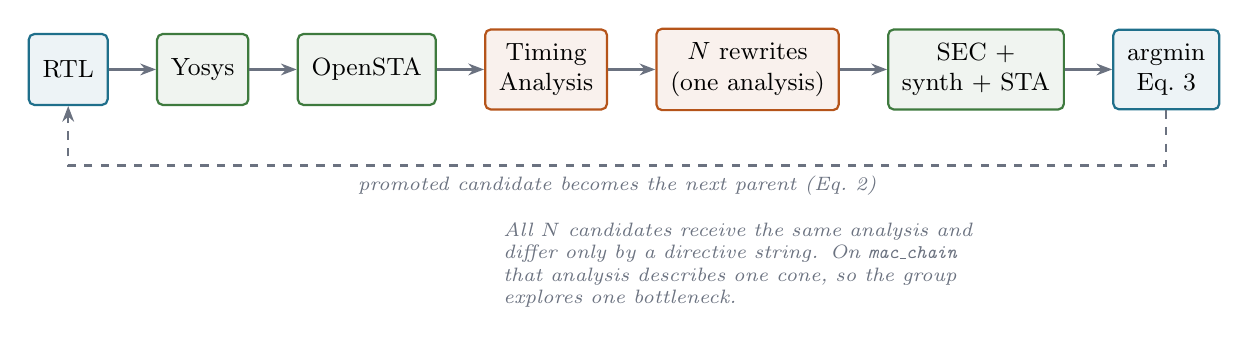
\begin{tikzpicture}[node distance=6mm]
  \node[stage] (rtl)   {RTL};
  \node[tool,  right=of rtl]  (syn)  {Yosys};
  \node[tool,  right=of syn]  (sta)  {OpenSTA};
  \node[llm,   right=of sta]  (an)   {Timing\\Analysis};
  \node[llm,   right=of an]   (opt)  {$N$ rewrites\\(one analysis)};
  \node[tool,  right=of opt]  (ev)   {SEC $+$\\synth $+$ STA};
  \node[stage, right=of ev]   (sel)  {argmin\\Eq.~3};

  \foreach \a/\b in {rtl/syn, syn/sta, sta/an, an/opt, opt/ev, ev/sel}
    \draw[flow] (\a) -- (\b);
  \draw[dashflow] (sel.south) -- ++(0,-7mm) -| node[note, pos=0.25, below]
        {promoted candidate becomes the next parent (Eq.~2)} (rtl.south);

  \node[note, below=13mm of opt, text width=6.2cm]
       {All $N$ candidates receive the same analysis and differ only by a
        directive string. On \texttt{mac\_chain} that analysis describes one
        cone, so the group explores one bottleneck.};
\end{tikzpicture}
\caption{The Dr.\ RTL loop, and where its exploration collapses.}
\label{fig:drrtl}
\end{figure}

% =====================================================================
\section{The pipeline}

Figure~\ref{fig:pipeline} shows the addon. Three stages are new; evaluation,
scoring, equivalence checking and skill learning are reused unchanged.

\begin{figure}[t]
\centering
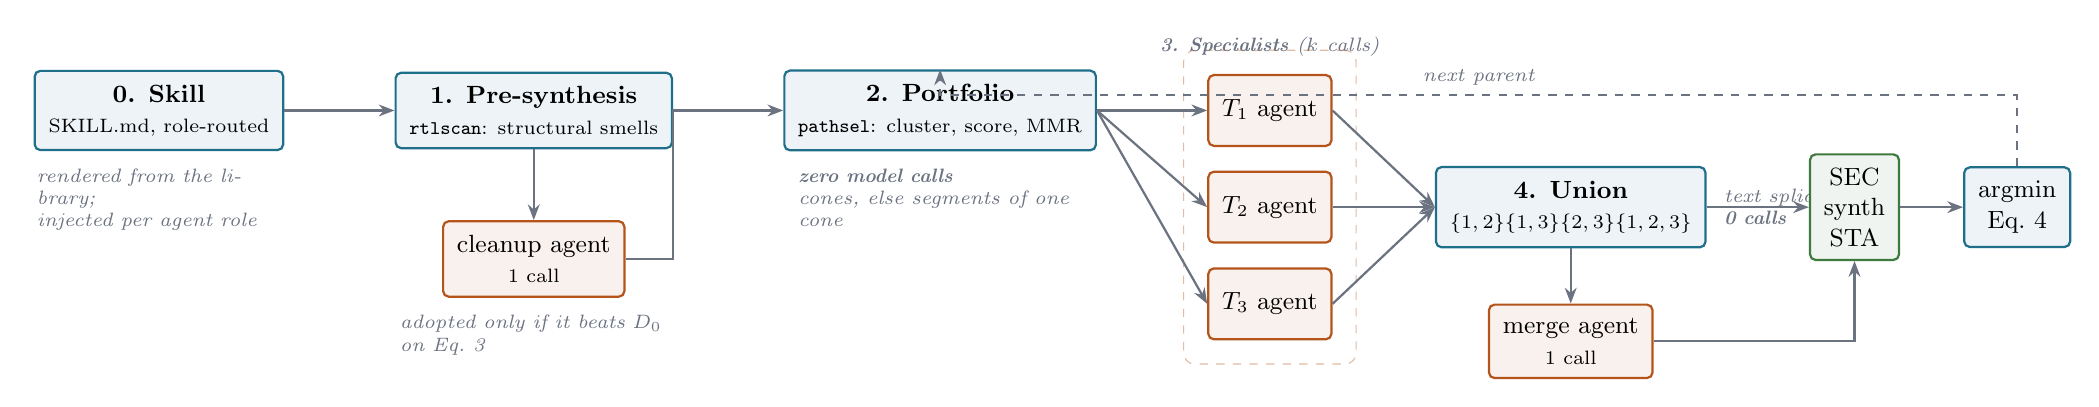
\begin{tikzpicture}[node distance=5mm and 7mm]

% ---- stage 0 -------------------------------------------------------
\node[stage] (skill) {\textbf{0. Skill}\\ \scriptsize SKILL.md, role-routed};
\node[note, below=1mm of skill, text width=3.1cm]
     {rendered from the library;\\ injected per agent role};

% ---- stage 1 -------------------------------------------------------
\node[stage, right=14mm of skill] (scan) {\textbf{1. Pre-synthesis}\\
      \scriptsize \texttt{rtlscan}: structural smells};
\node[llm, below=9mm of scan] (clean) {cleanup agent\\ \scriptsize 1 call};
\node[note, below=1mm of clean, text width=3.4cm]
     {adopted only if it beats $D_0$\\ on Eq.~3};
\draw[flow] (scan) -- (clean);

% ---- stage 2 -------------------------------------------------------
\node[stage, right=14mm of scan] (sel) {\textbf{2. Portfolio}\\
      \scriptsize \texttt{pathsel}: cluster, score, MMR};
\node[note, below=1mm of sel, text width=3.6cm]
     {\textbf{zero model calls}\\ cones, else segments of one cone};

% ---- stage 3 -------------------------------------------------------
\node[llm, right=14mm of sel] (t1) {$T_1$ agent};
\node[llm, below=3mm of t1]   (t2) {$T_2$ agent};
\node[llm, below=3mm of t2]   (t3) {$T_3$ agent};
\node[note, above=1mm of t1] {\textbf{3. Specialists} ($k$ calls)};

% ---- stage 4 -------------------------------------------------------
\node[stage, right=13mm of t2] (mech) {\textbf{4. Union}\\
      \scriptsize $\{1,2\}\{1,3\}\{2,3\}\{1,2,3\}$};
\node[llm, below=7mm of mech] (mg) {merge agent\\ \scriptsize 1 call};
\node[note, right=1mm of mech, text width=2.5cm]
     {text splicing,\\ \textbf{0 calls}};

% ---- evaluation & selection ---------------------------------------
\node[tool, right=13mm of mech] (ev) {SEC\\ synth\\ STA};
\node[stage, right=8mm of ev] (eq4) {argmin\\ Eq.~4};

\draw[flow] (skill) -- (scan);
\draw[flow] (clean.east) -- ++(6mm,0) |- (sel.west);
\foreach \t in {t1,t2,t3} \draw[flow] (sel.east) -- (\t.west);
\foreach \t in {t1,t2,t3} \draw[flow] (\t.east) -- (mech.west);
\draw[flow] (mech) -- (mg);
\draw[flow] (mech.east) -- (ev.west);
\draw[flow] (mg.east) -| (ev.south);
\draw[flow] (ev) -- (eq4);

\draw[dashflow] (eq4.north) -- ++(0,9mm) -| node[note,pos=0.25,above]
      {next parent} (sel.north);

\begin{scope}[on background layer]
  \node[fit=(t1)(t3), draw=agent!40, dashed, rounded corners, inner sep=3mm] {};
\end{scope}
\end{tikzpicture}
\caption{The path-portfolio pipeline. Blue is mechanical, orange is a model
call, green is the EDA toolchain. Selection and the mechanical unions cost
nothing; the winner is chosen by measurement over
$\{\text{specialists}\}\cup\{\text{unions}\}\cup\{\text{parent}\}$.}
\label{fig:pipeline}
\end{figure}

% ---------------------------------------------------------------------
\subsection{Stage 0 --- the skill document}

Agents run with every tool denied, so a skill cannot be loaded the usual way;
the document is read from disk and concatenated into the system prompt. Each
section carries a marker naming the roles that need it, and the marker is
written into the document so a regenerated file carries its own routing.

\begin{center}
\begin{tabular}{@{}lrl@{}}
\toprule
role & injected & sections \\
\midrule
specialist & 3310 tok & all \\
cleanup    & 3015 tok & all but \emph{how to read a critical path} \\
merge      &  \textbf{504 tok} & invariants, wasted work, equivalence \\
\bottomrule
\end{tabular}
\end{center}

\noindent
The merge agent reconciles diffs between rewrites that already exist and never
invents a transformation, so the catalogue and path-reading material are cost
with no possible use. Routing saves roughly 2800 tokens per iteration at
$k=3$.

The document's most load-bearing section is the one naming what synthesis
\emph{already does} --- constant folding, common-subexpression elimination,
Boolean minimisation, trivial resource sharing, retiming --- because redoing
any of it in RTL changes no gates and still costs an equivalence proof. What
synthesis cannot do is change the algorithm, and that boundary is where an
agent's contribution actually lies.

% ---------------------------------------------------------------------
\subsection{Stage 2 --- portfolio selection}

Path selection is pure arithmetic over the parsed report. Paths are clustered
into logic cones by a weighted blend of RTL-region agreement, cone-origin net
overlap, cell-family divergence and endpoint agreement:
%
\begin{equation}
\mathrm{sim}(p,q) \;=\;
  0.30\, J_w(R_p,R_q) \;+\;
  0.40\, J(O_p,O_q)   \;+\;
  0.20\, H(F_p,F_q)   \;+\;
  0.10\, E(p,q),
\end{equation}
%
with $J_w$ a weighted Jaccard over region delay shares, $J$ a Jaccard over
cone-origin nets, $H = 1 - \tfrac12\|F_p-F_q\|_1$ over normalised cell-family
histograms, and $E$ an endpoint/startpoint indicator. A term for which neither
path has evidence is dropped and the remaining weights renormalised; scoring
absent evidence as dissimilarity made a path only $0.70$ similar to itself on
any design where localisation fails.

Cone origins carry the largest weight because they are the only term measured
to discriminate on a real report: region sets came back at $J=1.00$ across
every pair of the reference design's twenty paths, while cone origins --- which
retain the bit index, so \texttt{acc\_out[9]} and \texttt{acc\_out[36]} stay
distinct points in one cone --- spread across $0.79$ to $0.96$.

\paragraph{Which path limits the clock.}
Static timing analysis is deterministic, so this is \emph{not} a probability
that the design fails, and not statistical STA over process variation. It
answers a question that is genuinely open before layout: post-synthesis timing
carries no real wire delay, so two paths a few picoseconds apart are not yet
reliably ordered, and committing $k$ agents to the nominally worst one is a bet
on an ordering the flow has not established. Each path delay is sampled as
%
\begin{equation}
d_i \;=\; -s_i \;+\; \sigma\!\left(\sqrt{\rho}\, z_{c(i)} \;+\; \sqrt{1-\rho}\, z_i\right),
\qquad z \sim \mathcal{N}(0,1),
\end{equation}
%
with $s_i$ the reported slack, $\sigma$ a fraction of the clock period, and
$\rho$ the share of the uncertainty common to a whole cone. The cone term is
load-bearing: without it, twenty bit-slices of one bottleneck each take
$1/20$ of the criticality and the cone owning all of it looks unimportant.
$P(\text{$i$ limits the clock})$ is then estimated by Monte Carlo with a fixed
seed. Setting $\sigma=0$ recovers the deterministic answer exactly.

Using slack rather than arrival means this works unchanged on a design that
\emph{meets} timing --- the case that arises whenever the goal is a tighter
period rather than a repair.

\begin{center}
\captionof{table}{Sensitivity: two cones 15\,ps apart.}
\begin{tabular}{@{}lrr@{}}
\toprule
$\sigma$ (of period) & cone A ($+0.100$) & cone B ($+0.115$) \\
\midrule
$0$ (deterministic) & 100\,\% & 0\,\% \\
$0.01$ & 71\,\% & 29\,\% \\
$0.05$ (default) & 55\,\% & 45\,\% \\
$0.20$ & 51\,\% & 49\,\% \\
\bottomrule
\end{tabular}
\end{center}

\paragraph{Value and selection.}
Each cluster is scored on three terms in $[0,1]$:
%
\begin{equation}
V(C) = 0.45\,\underbrace{P_{\mathrm{crit}}(C)}_{\text{impact}}
     + 0.35\,\underbrace{\tfrac12\!\left(1-\tfrac{s_C}{T}\right)}_{\text{severity}}
     + 0.20\,\underbrace{\tau(C)}_{\text{tractability}},
\end{equation}
%
where $T$ is the clock period and severity is clipped to $[0,1]$, placing the
constraint itself at $0.5$ so the term is monotone in delay on both sides of
zero slack. Tractability combines RTL localisation coverage, whether a
structural heuristic fired, and whether the skill library recognises the
shape; it is what stops the portfolio spending an agent on a path nobody can
act on. Targets are then chosen by maximal marginal relevance,
%
\begin{equation}
C^\star = \arg\max_{C}\;\Big[(1-\lambda)\,V(C) \;-\; \lambda \max_{S \in \mathcal{S}} \mathrm{sim}(C,S)\Big],
\end{equation}
%
so the second target is the best one that is also \emph{different} from the
first.

\paragraph{$k$ is a ceiling, not a quota.}
A design with one cone yields one target. Where fewer cones exist than agents,
the best cone's representative path is cut into contiguous \emph{segments} at
the points where its cell-family signature changes. On \texttt{mac\_chain} this
recovers the three bottlenecks the design declares by hand in its
configuration --- without ever reading that field (Table~\ref{tab:segments}).

\begin{table}[t]
\centering
\caption{Segments recovered from the STA report alone, against the
bottlenecks \texttt{mac\_chain/config.json} declares by hand.}
\label{tab:segments}
\begin{tabular}{@{}llrlp{5.1cm}@{}}
\toprule
target & stages & delay & cell signature & declared bottleneck \\
\midrule
$T_1$ & 0--24  & 36\,\% & 18$\times$ AND/OR, \textbf{fanout 42} & four unpipelined $16\times16$ multipliers \\
$T_2$ & 24--50 & 28\,\% & 14$\times$ AOI/OAI, 12$\times$ XOR & serial adder chain (carry propagation) \\
$T_3$ & 50--91 & 36\,\% & 36$\times$ AOI/OAI & 40-bit saturation compare \\
\bottomrule
\end{tabular}
\end{table}

% ---------------------------------------------------------------------
\subsection{Stage 4 --- recombination}

Two questions follow from $k$ independent rewrites, and only the second needs a
model: whether their edits touch disjoint text (diff arithmetic), and when they
do not, which fix wins (judgement).

Every subset of the surviving candidates that composes by text splicing is
assembled and evaluated --- four extra fully-measured designs per iteration for
zero model calls. Two properties are load-bearing and tested. The union is
\emph{order independent}: a region two candidates both edited is dropped whole
rather than resolved last-writer-wins, because a control whose result changes
when its inputs are shuffled is not a control. And a candidate that reformatted
the file is detected by its changed-line fraction and excluded with the reason
recorded, rather than making every other candidate conflict with it.

Final selection is Eq.~4 over
$\{\text{specialists}\} \cup \{\text{mechanical unions}\} \cup \{\text{agent
union}\} \cup \{\text{parent}\}$. A union does not win for being a union:
combined fixes can trip the area penalty, or expose a fourth path neither agent
saw. The mechanical unions double as the control on the merge agent, and every
summary reports
$\mathrm{score}(\text{agent}) - \mathrm{score}(\text{best mechanical})$.

% =====================================================================
\section{Measured results}

All runs use Haiku as the agent model on \texttt{mac\_chain} at a 2\,ns target,
Yosys for synthesis and OpenSTA for timing.

\begin{table}[h]
\centering
\caption{Measured outcomes. Score is Eq.~3 relative to $D_0$; lower is better.
SEC is counted over candidates that reached a verdict.}
\label{tab:results}
\begin{tabular}{@{}lrrrrrr@{}}
\toprule
run & iters & calls & $\Delta$WNS & $\Delta$TNS & Eq.~3 & SEC \\
\midrule
Dr.\ RTL baseline            & 3 & 18 & \textbf{+54.7\,\%} & +58.7\,\% & $-0.4789$ & 11/12 \\
portfolio                    & 2 & 11 & +53.5\,\% & +56.7\,\% & $-0.4658$ & 4/6 \\
portfolio (extended)         & 3 &  5 & +47.1\,\% & \textbf{+79.8\,\%} & $\mathbf{-0.5153}$ & 3/3 \\
portfolio, 1 iteration       & 1 &  6 & +52.8\,\% & +56.0\,\% & $-0.4599$ & 3/3 \\
\bottomrule
\end{tabular}
\end{table}

\noindent
The portfolio wins on total negative slack and on the composite Eq.~3
objective; the base loop wins on worst negative slack. Equivalence pass rates
are comparable (13/15 against 11/12 across all portfolio runs). One portfolio
iteration reaches within two percentage points of the base loop's
three-iteration WNS at a third of the model calls.

Two caveats. The extended run lost six of nine model calls to CLI failures, so
it is not a clean data point. And the skill library was shared across arms,
which advantages whichever ran second.

% =====================================================================
\section{Defects the measurements exposed}

Three findings, each a case where the instrument was wrong rather than the
method.

\paragraph{The equivalence pass rate was mis-counted.}
Both loops reported $\text{passed}/\text{attempted}$, so a candidate the model
never produced --- a CLI failure, a reply with no Verilog in it --- was recorded
as an \emph{equivalence failure}. On one run this reported three of three
candidates passing as 33\,\%, because six of nine calls had died before writing
anything: a property of the harness presented as a property of the method. The
codebase already distinguished refuted from undecided; the reporting ignored it.

\paragraph{The skill library fragmented its own evidence.}
An agent declined a transformation citing a library entry whose own recorded
advantage was favourable. One concept --- high fanout on a multiplier operand
--- had forked into four entries of one or two trials each, none able to clear
the support term, and one carried a \emph{verdict} where its strategy should
have been (``register replication already attempted; insufficient margin'').
Three causes: literal token matching (\texttt{register} and \texttt{registers}
scored as unrelated), Jaccard punishing verbosity, and no guard against a
conclusion being stored as a transformation. After repair the concept is a
single entry at $n=5$, confidence $0.46$, mean advantage $-0.53$.

\paragraph{Segmentation does not imply RTL separability.}
Run without the pre-synthesis stage, all three specialists made the
\emph{same} edit --- rebalancing the serial adder chain --- and produced
identical measurements. Every hunk then contested every other, so the
mechanical union returned the parent unchanged. With the pre-synthesis stage
enabled, the same configuration produced three distinct patterns and three
distinct scores.

This inverts the role of stage~1. It is not optional garnish: by taking the
obvious fix off the table, it is what forces the specialists onto genuinely
different bottlenecks. A path being separable into segments does not make the
RTL separable, and on this design the highest-value fix is reachable from every
segment.

% =====================================================================
\section{What remains undemonstrated}

\begin{itemize}\itemsep2pt
\item \textbf{Cone selection has never fired.} Neither shipped design can
      exercise it: \texttt{mac\_chain} is one cone, \texttt{alu32} meets
      timing. A third design (\texttt{dual\_path}, two unrelated slow
      datapaths sharing only the clock) exists for this and has not been
      synthesised. Until then the cone half of the selector is asserted, not
      shown.
\item \textbf{Segmentation has a validation set of one.} It reproduces
      \texttt{mac\_chain}'s hand-declared bottlenecks, which is suggestive,
      not proof.
\item \textbf{The merge agent has not earned its call.} Its measured delta
      against the free mechanical union is $0.0000$ on every run so far.
\item \textbf{Post-place-and-route is not built.} The stage parameter exists
      and \texttt{--stage pnr} reads the right report; the second pass over it
      is not wired up.
\item \textbf{Open-source synthesis is the ceiling.} Yosys is weaker than
      commercial synthesis, which both inflates trivial rewrites and can
      flatten real restructuring. A slack win here is a smaller claim than the
      same number elsewhere.
\end{itemize}

% =====================================================================
\section{Cost}

\begin{center}
\begin{tabular}{@{}lr@{}}
\toprule
step & model calls \\
\midrule
portfolio selection & \textbf{0} (arithmetic) \\
specialists & $k$ \\
mechanical unions, and evaluating them & \textbf{0} \\
merge agent & 1 \\
skill learning & 1 \\
\midrule
per iteration & $k+2 = 5$ \\
\bottomrule
\end{tabular}
\end{center}

\noindent
Defaults ($k=3$, 3 iterations, one cleanup call) plan 16 calls against the base
loop's 18. The plan is printed before anything runs and written to
\texttt{budget.json}; \texttt{--max-calls} refuses to start over budget.

% =====================================================================
\section{Reproducing}

\begin{lstlisting}
make skilldoc                                     # build SKILL.md
make scan  DESIGN=mac_chain                       # pre-synthesis smells
make paths DESIGN=mac_chain RUN=<run-id>          # the portfolio, no model
make portfolio DESIGN=mac_chain PF_ARGS="--model haiku"

# head-to-head; reset the library between arms or the second inherits
make clean-skills
make opt       DESIGN=mac_chain OPT_ARGS="--model haiku"
make clean-skills
make portfolio DESIGN=mac_chain PF_ARGS="--model haiku"
\end{lstlisting}

\noindent
Selection is checkable with no tools and no model against the committed run
artifact:

\begin{lstlisting}
python3 tools/pathsel.py results/mac_chain/opt-20260915-103411/baseline -k 3
python3 tools/selftest.py     # 162 tests, no EDA install required
\end{lstlisting}

\end{document}
